\achapter{28}{Quadratic Forms and the Principal Axis Theorem} \label{chap:principal_axis_theorem}

\vspace*{-17 pt}
\framebox{\hspace*{3 pt}
\parbox{4.7 in}{\begin{fqs}
\item What is a quadratic form on $\R^n$?
\item What does the Principal Axis Theorem tell us about quadratic forms? 
\end{fqs}} \hspace*{3 pt}}

\vspace*{3 pt}

\csection{Application: The Tennis Racket Effect} 
\label{sec:appl_tennis}

Try an experiment with a tennis racket (or a squash racket, or a ping pong paddle). Let us define a 3D coordinate system with the center of the racket as the origin with the head of the racket lying in the $xy$-plane. We let $\vu_1$ be the vector in the direction of the handle and $\vu_2$ the perpendicular direction (still lying in the plane defined by the head) as illustrated in Figure \ref{F:tennis_racket}. We then let $\vu_3$ be a vector perpendicular to the plane of the head. Hold the racket by the handle and spin it to make one rotation around the $\vu_1$ axis. This is pretty easy. It is also not difficult to throw the racket so that it rotates around the $\vu_3$. Now toss the racket into the air to make one complete rotation around the axis of the vector $\vu_2$ and catch the handle. Repeat this several times. You should notice that in most instances, the racket will also have made a half rotation around the $\vu_1$ axis so that the other face of the racket now points up. This is quite different than the rotations around the $\vu_1$ and $\vu_3$ axes. A good video that illustrates this behavior can be seen at \url{https://www.youtube.com/watch?v=4dqCQqI-Gis}. 

\begin{figure}[ht]
  \begin{center}
\resizebox{!}{1.0in}{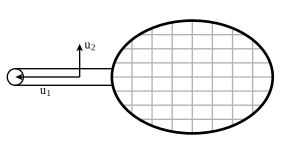
\includegraphics{7_b_tennis_racket.eps}} 
    \caption{Two principal axes of a tennis racket.}
    \label{F:tennis_racket}
  \end{center}
\end{figure}

This effect is a result in classical mechanics that describes the rotational movement of a rigid body in space, called the \emph{tennis racket effect} (or the Dzhanibekov effect, after the Russian cosmonaut Vladimir Dzhanibekov who discovered the theorem's consequences while in zero gravity in space -- you can see an illustration of this in the video at \url{https://www.youtube.com/watch?v=L2o9eBl_Gzw}). The result is simple to see in practice, but is difficult to intuitively understand why the behavior is different around the intermediate axis. There is a story of a student who asked the famous physicist Richard Feynman if there is any intuitive way to understand the result; Feynman supposedly went into deep thought for about 10 or 15 seconds and answered, "no." As we will see later in this section, we can understand this effect using the principal axes of a rigid body. 

\csection{Introduction}
\label{sec:pat_intro}

We are familiar with quadratic equations in algebra. Examples of quadratic equations include $x^2=1$, $x^2+y^2=1$, and $x^2+xy+y^2=3$. We don't, however, have to restrict ourselves to two variables. A quadratic equation in $n$ variables is any equation in which the sum of the exponents in any monomial term is 2. So a quadratic equation in the variables $x_1$, $x_2$, $\ldots$, $x_n$ is an equation in the form
\begin{align*}
a_{11}x_1^2&+a_{22}x_2^2 + a_{33}x_3^2 + \cdots + a_{nn}x_n^2 \\
	&+ a_{12}x_1x_2 + a_{13}x_1x_3 + \cdots a_{1n}x_1x_n \\
	&+ a_{23}x_2x_3 + a_{24}x_2x_4 + \cdots a_{2n}x_2x_n + \cdots  \\
	&+ a_{n-1n}x_{n-1}x_n \\
	&= c
\end{align*}
for some constant $c$. In matrix notation this expression on the left of this equation has the form
\[\sum_{i=1}^{n} \sum_{j=1}^n a_{ij}x_ix_j = \vx^{\tr} A \vx\]
where $\vx = \left[ \begin{array}{c} x_1 \\ x_2 \\ \vdots \\ x_n \end{array} \right]$ and $A$ is the $n \times n$ matrix $A = [a_{ij}]$. For example, if $A= \left[ \begin{array}{rcr} 1&3&-2 \\ -1&1&2 \\ 0&2&-2\end{array} \right]$, then we get the quadratic expression $x_1^2+3x_1x_2-2x_1x_3-x_2x_1+x_2^2+2x_2x_3+2x_3x_2-2x_3^2$. We should note here that the terms involving $x_ix_j$ and $x_jx_i$ are repeated in our sum, but
\[a_{ij}x_ix_j + a_{ji}x_jx_i = 2\left(\frac{a_{ij} + a_{ji}}{2}\right)x_ix_j\]
and so we could replace $a_{ij}$ and $a_{ji}$ both with $\left(\frac{a_{ij} + a_{ji}}{2}\right)$ without changing the quadratic form. With this alteration in mind, we can then assume that $A$ is a symmetric matrix. So in the previous example, the symmetric matrix $A'= \left[ \begin{array}{rcr} 1&1&-1 \\ 1&1&2 \\ -1&2&-2\end{array}\right]$ gives the same quadratic expression. This leads to the following definition.


\begin{definition} A \textbf{quadratic form}\index{quadratic form} on $\R^n$ is a function $Q$ defined by
\[Q(\vx) = \vx^{\tr} A \vx\]
for some $n \times n$ symmetric matrix $A$.
\end{definition}


As we show in Exercise \ref{ex:7_b_unique_A}, the symmetric matrix $A$ is unique to the quadratic form, so we call the symmetric matrix $A$ is the \emph{matrix of the quadratic form}. It is these quadratic forms that we will study in this section.

\begin{pa} \label{pa:7_b}  ~
\be
\item To get a little more comfortable with quadratic forms, write the quadratic forms in matrix form, explicitly identifying the vector $\vx$ and the symmetric matrix $A$ of the quadratic form.
	\ba
	\item $3x_1^2-2x_2^2 +4x_1x_2+x_2x_3$ 

	\item  $x_1x_4 + 4x_2x_3 - x_2^2 + 10x_1x_5$ 

	\ea

\item Some quadratic forms form equations in $\R^2$ that are very familiar: $x^2+y^2=1$ is an equation of a circle, $2x^2+3y^2=2$ is an equation of an ellipse, and $x^2-y^2=1$ is an equation of a hyperbola. Of course, these do not represent all of the quadratic forms in $\R^2$ -- some contain cross-product terms. We can recognize the equations above because they contain no cross-product terms (terms involving $xy$). We can more easily recognize the quadratic forms that contain cross-product terms if  we can somehow rewrite the forms in a different format with no cross-product terms. We illustrate how this can be done with the quadratic form $Q$ defined by $Q(\vx) = x^2-xy+y^2$. 
    \ba
    \item Write $Q(\vx)$ in the form $\vx^{\tr} A \vx$, where $A$ is a $2 \times 2 $ symmetric matrix.

    \item Since $A$ is a symmetric matrix we can orthogonally diagonalize $A$. Given that the eigenvalues of $A$ are $\frac{3}{2}$ and $\frac{1}{2}$ with corresponding eigenvectors $\left[ \begin{array}{r} -1 \\ 1 \end{array} \right]$ and $\left[ \begin{array}{c} 1 \\ 1 \end{array} \right]$, respectively, find a matrix $P$ that orthogonally diagonalizes $A$.

    \item Define $\vy = \left[ \begin{array}{c} w \\ z \end{array} \right]$ to satisfy $\vx = P\vy$. Substitute for $\vx$ in the quadratic form $Q(\vx)$ to write the quadratic form in terms of $w$ and $z$. What kind of graph does the quadratic equation $Q(\vx) = 1$ have?

    \ea
	

\ee

\end{pa} 



\csection{Equations Involving Quadratic Forms in $\R^2$}
\label{sec:eqs_quad_r2}

When we consider equations of the form $Q(\vx) = d$, where $Q$ is a quadratic form in $\R^2$ and $d$ is a constant, we wind up with old friends like $x^2+y^2=1$, $2x^2+3y^2=2$, or $x^2-y^2=1$. As we saw in Preview Activity \ref{pa:7_b} these equations are relatively easy to recognize. However, when we have cross-product terms, like in $x^2-xy+y^2=1$, it is not so easy to identify the curve the equation represents. If there was a way to eliminate the cross-product term $xy$ from this form, we might be more easily able to recognize its graph. The discussion in this section will focus on quadratic forms in $\R^2$, but we will see later that the arguments work in any number of dimensions. While working in $\R^2$ we will use the standard variables $x$ and $y$ instead of $x_1$ and $x_2$.

In general, the equation of the form $Q(\vx) = d$, where $Q$ is a quadratic form in $\R^2$ defined by a matrix $A = \left[ \begin{array}{cc} a&b/2\\b/2&c \end{array} \right] $ and $d$ is a constant looks like  
%\[d = Q(\vx) = \vx^{\tr}A \vx = [x \ y] \left[ \begin{array}{cc} a&b/2\\b/2&c \end{array} \right] \left[ \begin{array}{c} x\\y \end{array} \right] = ax^2+bxy+cy^2 = d.\]
\[ax^2+bxy+cy^2 = d.\]
The graph of an equation like this is either an ellipse (a circle is a special case of an ellipse), a hyperbola, two non-intersecting lines, a point, or the empty set (see Exercise \ref{ex:7_b_QF_characterization}). The quadratic forms do not involve linear terms, so we don't consider the cases of parabolas. One way to see into which category one of these quadratic form equations falls is to write the equation in standard form.

The standard forms for quadratic equations in $\R^2$ are as follows, where $a$ and $b$ are nonzero constants and $h$ and $k$ are any constants.
\begin{description}
\item[Lines:] $\ds ax^2 = 1$ or $\ds ay^2=1$ ($a > 0$)
\item[Ellipse: ] $\ds \frac{(x-h)^2}{a^2} + \frac{(y-k)^2}{b^2} = 1$
\item[Hyperbola: ] $\ds \frac{(x-h)^2}{a^2} - \frac{(y-k)^2}{b^2} = 1$  or $\ds \frac{(y-k)^2}{b^2} - \frac{(x-h)^2}{a^2} = 1$
%\item[Parabola: ] $(x-h)^2 = p(y-k)$ or $(y-k)^2 = p(x-h)$
\end{description}


Preview Activity \ref{pa:7_b} contains the main tool that we need to convert a quadratic form into one of these standard forms. By this we mean that if we have a quadratic form $Q$ in the variables $x_1$, $x_2$, $\ldots$, $x_n$, we want to find variables $y_1$, $y_2$, $\ldots$, $y_n$ in terms of $x_1$, $x_2$, $\ldots$, $x_n$ so that when written in terms of the variables $y_1$, $y_2$, $\ldots$, $y_n$ the quadratic form $Q$ contains no cross terms. In other words, we want to find a vector $\vy = \left[ \begin{array}{c} y_1 \\ y_2 \\ \vdots \\ y_n \end{array} \right]$ so that $Q(\vx) = \vy^{\tr} D \vy$, where $D$ is a diagonal matrix. Since every real symmetric matrix is orthogonally diagonalizable, we will always be able to find a matrix $P$ that orthogonally diagonalizes $A$.  The details are as follows. 

Let $Q$ be the quadratic form defined by $Q(\vx) = \vx^{\tr} A \vx$, where $A$ is an $n \times n$ symmetric matrix. As in Preview Activity \ref{pa:7_b}, the fact that $A$ is symmetric means that we can find an orthogonal matrix $P = [ \vp_1 \  \vp_2 \  \vp_3 \  \cdots \  \vp_n ]$ whose columns are orthonormal eigenvectors of $A$ corresponding to eigenvalues $\lambda_1$, $\lambda_2$, $\ldots$, $\lambda_n$, respectively. Letting $\vy = P^{\tr} \vx$ give us $\vx = P\vy$ and
\[\vx^{\tr} A \vx = (P\vy)^{\tr}A(P\vy) = \vy^{\tr}(P^{\tr}AP)\vy = \vy^{\tr} D \vy,\]
where $D$ is the diagonal matrix whose $i$th diagonal entry is $\lambda_i$.

Moreover, the set $\B = \{\vp_1, \vp_2, \cdots, \vp_n\}$ is an orthonormal basis for $\R^n$ and so defines a coordinate system for $\R^n$. Note that if $y = [y_1 \ y_2 \ \cdots \ y_n]^{\tr}$, then
\[\vx = P\vy = y_1\vp_1 + y_2 \vp_2 + \cdots + y_n \vp_n.\]
Thus, the coordinate vector of $\vx$ with respect to $\B$ is $\vy$, or $[\vx]_{\B} = \vy$. We summarize in Theorem \ref{thm:7_b_Principal_Axis_Theorem}. 

\begin{theorem}[Principal Axis Theorem] \label{thm:7_b_Principal_Axis_Theorem} Let $A$ be an $n \times n$ symmetric matrix. There is an orthogonal change of variables $\vx = P\vy$ so that the quadratic form $Q$ defined by $Q(\vx) = \vx^{\tr} A \vx$ is transformed into the quadratic form $\vy^{\tr} D \vy$ where $D$ is a diagonal matrix.
\end{theorem}

The columns of the orthogonal matrix $P$ in the Principal Axis Theorem form an orthogonal basis for $\R^n$ and are called the \emph{principal axes} for the quadratic form $Q$. Also, the coordinate vector of $\vx$ with respect to this basis is $\vy$.

\begin{activity} Let $Q$ be the quadratic form defined by $Q(\vx) = 2x^2 + 4xy + 5y^2 = \vx^{\tr} A \vx$, where $\vx = \left[ \begin{array}{c} x \\ y \end{array} \right]$ and $A = \left[ \begin{array}{cc}2&2\\2&5 \end{array} \right]$. 
    \ba


    \item The eigenvalues of $A$ are $\lambda_1 = 6$ and $\lambda_2=1$ with corresponding eigenvectors $\vv_1 = [1 \ 2]^{\tr}$ and $\vv_2 = [-2 \ 1]^{\tr}$, respectively. Find an orthogonal matrix $P$ with determinant 1 that diagonalizes $A$. Is $P$ unique? Explain. Is there a matrix without determinant 1 that orthogonally diagonalizes $A$? Explain.

    
    \item Use the matrix $P$ to write the quadratic form without the cross-product.

    \item We can view $P$ as a change of basis matrix from the coordinate system defined by $\vy = P^{\tr} \vx$ to the standard coordinate system. In other words, in the standard $xy$ coordinate system, the quadratic form is written as $\vx^{\tr}A \vx$, but in the new coordinate system defined by $\vy$ the quadratic form is written as $(P\vy)^{\tr}A(P\vy)$. As a change of basis matrix, $P$ performs a rotation. See if you can recall what we learned about rotation matrices and determine the angle of rotation $P$ defines. Plot the graph of the quadratic equation $Q(\vx) = 1$ in the new coordinate system and identify this angle on the graph. Interpret the result.

    \ea

\end{activity}

\csection{Classifying Quadratic Forms}
\label{sec:class_quad_forms}

If we draw graphs of equations of the type $z=Q(\vx)$, where $Q$ is a quadratic form, we can see that a quadratic form whose matrix does not have 0 as an eigenvalue can take on all positive values (except at $\vx=\vzero$) as shown at left in Figure \ref{F:7_b_Paraboloids}, all negative values (except at $\vx=\vzero$) as shown in the center of  Figure \ref{F:7_b_Paraboloids}, or both positive and negative values as depicted at right in Figure \ref{F:7_b_Paraboloids}. We can see when these cases happen by analyzing the eigenvalues of the matrix that defines the quadratic form. Let $A$ be a $2 \times 2$ symmetric matrix with eigenvalues $\lambda_1$ and $\lambda_2$, and let $P$ be a matrix that orthogonally diagonalizes $A$ so that $P^{\tr}AP = D = \left[ \begin{array}{cc} \lambda_1 & 0 \\ 0 & \lambda_2 \end{array} \right]$. If we let $\vy = \left[ \begin{array}{c} w\\z \end{array} \right] = P^{\tr}\vx$, then \begin{align*}
Q(\vx) &= \vx^{\tr}A\vx \\
	&= \vy^{\tr} D \vy \\
	&= \lambda_1 w^2 + \lambda_2 z^2.
\end{align*}
Then $Q(\vx) \geq 0$ if all of the eigenvalues of $A$ are positive (with $Q(\vx) > 0$ when $\vx \neq \vzero$) and $Q(\vx) \leq 0$  if all of the eigenvalues of $A$ are negative (with $Q(\vx) < 0$ when $\vx \neq \vzero$). If one eigenvalue of $A$ is positive and the other negative, then $Q(\vx)$ will take on both positive and negative values. As a result, we classify symmetric matrices (and their corresponding quadratic forms) according to these behaviors.
\begin{figure}[h]
\begin{center}
\resizebox{!}{1.5in}{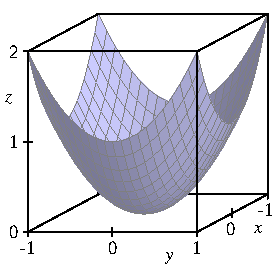
\includegraphics{7_b_Paraboloid}}
\resizebox{!}{1.5in}{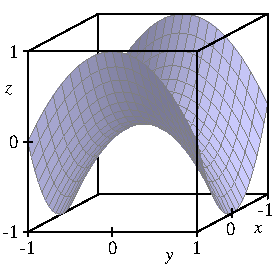
\includegraphics{7_b_Hyperbolic_Paraboloid}}
\resizebox{!}{1.5in}{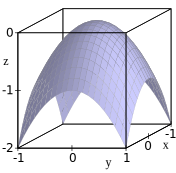
\includegraphics{7_b_Paraboloid2}}
\caption{Left: Paraboloid $Q(\vx)=x^2+y^2$. Center: Hyperbolic Paraboloid $Q(\vx)=x^2-y^2$. Right: Paraboloid $Q(\vx) = -x^2 - y^2$.}
\label{F:7_b_Paraboloids}
\end{center}
\end{figure}



\begin{definition} \label{def:7_4_definite} A symmetric matrix $A$ (and its associated quadratic form $Q$) is
\ba
\item \textbf{positive definite}\index{matrix!positive definite} if $\vx^{\tr}A\vx > 0$ for all $\vx \neq \vzero$,
\item \textbf{positive semidefinite}\index{matrix!positive semidefinite} if $\vx^{\tr}A\vx \geq 0$ for all $\vx$,
\item \textbf{negative definite}\index{matrix!negative definite} if $\vx^{\tr}A\vx < 0$ for all $\vx \neq \vzero$,
\item \textbf{negative semidefinite}\index{matrix!negative semidefinite} if $\vx^{\tr}A\vx \leq 0$ for all $\vx$,
\item \textbf{indefinite}\index{matrix!indefinite} if $\vx^{\tr}A\vx$ takes on both positive and negative values.
\ea
\end{definition}

For example, the quadratic form $Q(\vx) = x^2+y^2$ at left in Figure \ref{F:7_b_Paraboloids} is positive definite (with repeated eigenvalue 1), the quadratic form $Q(\vx) = -(x^2+y^2)$ at right in  Figure \ref{F:7_b_Paraboloids} is negative definite (repeated eigenvalue $-1$), and the hyperbolic paraboloid $Q(\vx) = x^2-y^2$ in the center of Figure \ref{F:7_b_Paraboloids} is indefinite (eigenvalues $1$ and $-1$). 

So we have argued that a quadratic form $Q(\vx) = \vx^{\tr} A \vx$ is positive definite if $A$ has all positive eigenvalues, negative definite if $A$ has all negative eigenvalues, and indefinite if $A$ has both positive and negative eigenvalues. Similarly, the quadratic form is positive semidefinite if $A$ has all nonnegative eigenvalues and negative semidefinite if $A$ has all nonpositive eigenvalues. Positive definite matrices are important, as we discuss in the next section.

\csection{Inner Products}
\label{sec:pat_inner_prod}

We used the dot product to define lengths of vectors, to measure angles between vectors, and to define orthogonality in $\R^n$. We can generalize the notion of orthogonality by using different types of products called \emph{inner products} that behave like the dot product. 

\begin{pa} \label{pa:7_b_inner_product} Define a  mapping from $\R^2 \times \R^2$ to $\R$ by
\[\langle \vu, \vv \rangle = u_1v_1 + 2u_2v_2\]
for $\vu = [u_1 \ u_2]^{\tr}$ and $\vv = [v_1 \ v_2]^{\tr}$ in $\R^2$. (The brackets $\langle \ \rangle$ provide a shorthand way of representing the function.) 
\be
\item Calculate $\langle [1 \ 2]^{\tr}, [3,-4]^{\tr} \rangle$. 
	
\item If $\vu$ and $\vv$ are in $\R^2$, is it true that 
	\[ \langle \vu , \vv \rangle = \langle \vv , \vu \rangle?\]
	Verify your answer.
	
\item If $\vu$, $\vv$, and $\vw$ are in $\R^2$, is it true that 
	\[\langle \vu + \vv , \vw \rangle = \langle \vu , \vw \rangle + \langle \vv , \vw \rangle?\]
	Verify your answer.
	
\item If $\vu$ and $\vv$ are in $\R^2$ and $c$ is a scalar, is it true that 
\[\langle c\vu , \vv \rangle = c\langle \vu , \vv \rangle?\]
Verify your answer. 

\item If $\vu$ and $\vv$ are in $\R^2$, must it be the case that $\langle \vu , \vu \rangle \geq 0$? When is $\langle \vu , \vu \rangle = 0$?

\item There is a matrix $A$ such that $\langle \vu, \vv \rangle = \vu^{\tr} A \vv$. Find this matrix $A$.
 
\ee

\end{pa}

Preview Activity \ref{pa:7_b_inner_product} illustrates that there are functions from $\R^n \times \R^n$ to $\R$ other than the dot product that satisfy many of the properties in Theorem \ref{thm:6_a_dot_product}. Such functions allow us to broaden our ideas of what right angles look like. These functions are called \emph{inner products}. 

\begin{definition} \label{def:7_b_inner_product}  An \textbf{inner product}\index{inner product} $\langle \ , \ \rangle$ on $\R^n$ is a mapping from $\R^n \times \R^n \to \R$ satisfying
\begin{enumerate}
\item $\langle \vu , \vv \rangle = \langle \vv , \vu \rangle$ for all $\vu$ and $\vv$ in $\R^n$,
\item $\langle \vu + \vv , \vw \rangle = \langle \vu , \vw \rangle + \langle \vv , \vw \rangle$ for all $\vu$, $\vv$, and $\vw$ in $\R^n$,
\item $\langle c\vu , \vv \rangle = c\langle \vu , \vv \rangle$ for all $\vu$, $\vv$ in $\R^n$ and all scalars $c$,
\item $\langle \vu , \vu \rangle \geq 0$ for all $\vu$ in $\R^n$ and $\langle \vu , \vu \rangle = 0$ if and only if $\vu = \vzero$.
\end{enumerate}
\end{definition}   

The dot product and the example in Activity \ref{pa:7_b_inner_product} provide two examples of inner products. The examples below provide two other important inner products on $\R^n$.

\begin{itemize}
\item If $a_1$, $a_2$, $\ldots$, $a_n$ are positive scalars, then 
\[\langle [u_1 \ u_2 \ \cdots \ u_n]^{\tr},  [v_1 \ v_2 \ \cdots \ v_n]^{\tr} \rangle = a_1u_1v_1+a_2u_2v_2+ \cdots + a_nu_nv_n\]
 defines an inner product on $\R^n$. 
\item Every invertible $n \times n$ matrix $A$ defines an inner product on $\R^n$ by  
\[\langle \vu, \vv \rangle = (A\vu) \cdot (A\vv).\]
\end{itemize}

As Exercise \ref{ex:7_b_PD_inner_product} will demonstrate, every inner product on $\R^n$ can be written in the form $\langle \vu, \vv \rangle = \vu^{\tr} A \vv$ for some special type of matrix $A$. 

\begin{activity} Let $A$ be a symmetric $n \times n$ matrix, and define $\langle \ , \ \rangle : \R^n \times \R^n \to \R$ by
    \begin{equation} \label{eq:7_b_PD_inner_product}
    \langle \vu, \vv \rangle = \vu^{\tr}A\vv.
    \end{equation}
    \ba
    \item Explain why it is necessary for $A$ to be positive definite in order for (\ref{eq:7_b_PD_inner_product}) to define an inner product on $\R^n$.

    \item Show that (\ref{eq:7_b_PD_inner_product}) defines an inner product on $\R^n$ if $A$ is positive definite.

	\item Let $\langle \ , \ \rangle$ be the mapping from $\R^2\times \R^2\to \R$ defined by
\[\left\langle \left[ \begin{array}{c} x_1 \\ x_2 \end{array} \right], \left[ \begin{array}{c} y_1 \\ y_2 \end{array} \right] \right\rangle = 2x_1y_1 - x_1y_2 - x_2y_1 + x_2y_2.\]
Find a matrix $A$ so that $\langle \vx, \vy \rangle = \vx^{\tr} A \vy$ and explain why $\langle \ , \ \rangle$ defines an inner product. 

    \ea

\end{activity}

\csection{Examples}
\label{sec:pat_exam}

\ExampleIntro

\begin{example} Write the given quadratic equation in a system in which it has no cross-product terms.
	\ba
	\item $8x^2-4xy+5y^2 = 1$
	
	\item $x^2+4xy+y^2=1$

	\item $4x^2+4y^2+4z^2+4xy+4xz+4yz-3=0$

	\ea

\ExampleSolution
	\ba
	\item We write the quadratic form $Q(x,y)=8x^2-4xy+5y^2$ as $\vx^{\tr} A \vx$, where $\vx = \left[ \begin{array}{c} x\\y \end{array} \right]$ and $A = \left[  \begin{array}{rr} 8&-2\\-2&5 \end{array} \right]$. The eigenvalues for $A$ are $9$ and $4$, and bases for the corresponding eigenspaces $E_9$ and $E_{4}$ are $\{[-2 \ 1]^{\tr}\}$ and $\{[1 \ 2]^{\tr}\}$, respectively. An orthogonal matrix $P$ that orthogonally diagonalizes $A$ is 
\[P = \left[\renewcommand{\arraystretch}{1.2} \begin{array}{rc} -\frac{2}{\sqrt{5}}&\frac{1}{\sqrt{5}} \\ \frac{1}{\sqrt{5}}&\frac{2}{\sqrt{5}}  \end{array} \right].\]
If $\vy =  [u \ v]^{\tr}$ and we let $\vx = P\vy$, then we can rewrite the quadratic equation $8x^2-4xy+5y^2 = 1$ as 
\begin{align*}
8x^2-4xy+5y^2 &= 1 \\
\vx^{\tr}A\vx &= 1 \\
(P\vy)^{\tr}A(P\vy) &= 1 \\
\vy^{\tr} P^{\tr}AP \vy &= 1 \\
\vy^{\tr} \left[ \begin{array}{cc} 9&0\\0&4 \end{array} \right] \vy &= 1 \\
9u^2+4v^2 &= 1.
\end{align*}
So the quadratic equation $8x^2-4xy+5y^2=1$ is an ellipse.   
 
	\item We write the quadratic form $Q(x,y)=x^2+4xy+y^2$ as $\vx^{\tr} A \vx$, where $\vx = \left[ \begin{array}{c} x\\y \end{array} \right]$ and $A = \left[  \begin{array}{cc} 1&2\\2&1 \end{array} \right]$. The eigenvalues for $A$ are $3$ and $-1$, and bases for the corresponding eigenspaces $E_3$ and $E_{-1}$ are $\{[1 \ 1]^{\tr}\}$ and $\{[-1 \ 1]^{\tr}\}$, respectively. An orthogonal matrix $P$ that orthogonally diagonalizes $A$ is 
\[P = \left[\renewcommand{\arraystretch}{1.2} \begin{array}{rc} \frac{1}{\sqrt{2}}&\frac{1}{\sqrt{2}} \\ -\frac{1}{\sqrt{2}}&\frac{1}{\sqrt{2}}  \end{array} \right].\]
If $\vy =  [u \ v]^{\tr}$ and we let $\vx = P\vy$, then we can rewrite the quadratic equation $x^2+4xy+y^2 = 1$ as 
\begin{align*}
x^2+4xy+y^2 &= 1 \\
\vx^{\tr}A\vx &= 1 \\
(P\vy)^{\tr}A(P\vy) &= 1 \\
\vy^{\tr} P^{\tr}AP \vy &= 1 \\
\vy^{\tr} \left[ \begin{array}{cr} 3&0\\0&-1 \end{array} \right] \vy &= 1 \\
3u^2-v^2 &= 1.
\end{align*}
So the quadratic equation $x^2+4xy+y^2=1$ is a hyperbola.  
 
	\item  We write the quadratic form $Q(x,y,z)=4x^2+4y^2+4z^2+4xy+4xz+4yz$ as $\vx^{\tr} A \vx$, where $\vx = \left[ \begin{array}{c} x\\y\\z \end{array} \right]$ and $A = \left[ \begin{array}{ccc} 4&2&2\\2&4&2\\2&2&4 \end{array} \right]$. The eigenvalues for $A$ are $2$ and $8$, and bases for the corresponding eigenspaces $E_2$ and $E_8$ are $\{[-1 \ 0 \ 1]^{\tr}, [-1 \ 1\ 0]^{\tr}\}$ and $\{[1 \ 1\ 1]^{\tr}\}$, respectively. Applying the Gram-Schmidt process to the basis for $E_2$ gives us an orthogonal basis $\{\vw_1, \vw_2\}$ of $E_2$, where $\vw_1 = [-1 \ 0 \ 1]^{\tr}$ and 
\begin{align*}
\vw_2 &=  [-1 \ 1 \ ]^{\tr} - \frac{ [-1 \ 0 \ 1]^{\tr} \cdot [-1 \ 1 \ 0]^{\tr}}{[-1 \ 0 \ 1]^{\tr} \cdot [-1 \ 0 \ 1]^{\tr}} [-1 \ 0 \ 1]^{\tr} \\
	&=  [-1 \ 1 \ 0]^{\tr} - \frac{1}{2}[-1 \ 0 \ 1]^{\tr} \\
	&= \frac{1}{2}[ -1 \ 2 \ -1]^{\tr}.
\end{align*}
An orthogonal matrix $P$ that orthogonally diagonalizes $A$ is 
\[P = \left[\renewcommand{\arraystretch}{1.2} \begin{array}{rrc} -\frac{1}{\sqrt{2}}&-\frac{1}{\sqrt{6}}&\frac{1}{\sqrt{3}} \\ 0&\frac{2}{\sqrt{6}}&\frac{1}{\sqrt{3}} \\ \frac{1}{\sqrt{2}}&-\frac{1}{\sqrt{6}}&\frac{1}{\sqrt{3}} \end{array} \right].\]
If $\vy =  [u \ v \ w]^{\tr}$ and we let $\vx = P\vy$, then we can rewrite the quadratic equation $4x^2+4y^2+4z^2+4xy+4xz+4yz = 3$ as 
\begin{align*}
4x^2+4y^2+4z^2+4xy+4xz+4yz &= 3 \\
\vx^{\tr}A\vx &= 3 \\
(P\vy)^{\tr}A(P\vy) &= 3 \\
\vy^{\tr} P^{\tr}AP \vy &= 3 \\
\vy^{\tr} \left[ \begin{array}{ccc} 2&0&0\\0&2&0\\0&0&8 \end{array} \right] \vy &= 3 \\
2u^2+2v^2+8w^2 &= 3.
\end{align*}
So the quadratic equation $4x^2+4y^2+4z^2+4xy+4xz+4yz-3 = 0$ is a ellipsoid.  

	\ea


\end{example}

\begin{example} Let $A$ and $B$ be positive definite matrices, and let $C = \left[ \begin{array}{rr}5&-3\\-3&3 \end{array} \right]$. 
\ba
\item Must $A$ be invertible? Justify your answer. 

\item Must $A^{-1}$ be positive definite? Justify your answer. 

\item Must $A^{2}$ be positive definite? Justify your answer. 

\item Must $A+B$ be positive definite? Justify your answer. 

\item Is $C$ positive definite? Justify your answer. 

\ea

\ExampleSolution

\ba
\item Since $A$ has all positive eigenvalues and $\det(A)$ is the product of the eigenvalues of $A$, then $\det(A) > 0$. Thus, $A$ is invertible.

\item The fact that $A$ is positive definite means that $A$ is also symmetric. Recall that $\left(A^{-1}\right)^{\tr} = \left(A^{\tr}\right)^{-1}$. Since $A$ is symmetric, it follows that $\left(A^{-1}\right)^{\tr} = A^{-1}$ and $A^{-1}$ is symmetric. The eigenvalues of $A^{-1}$ are the reciprocals of the eigenvalues of $A$. Since the eigenvalues of $A$ are all positive, so are the eigenvalues of $A^{-1}$. Thus, $A^{-1}$ is positive definite.

\item Notice that 
\[\left(A^2\right)^{\tr} = (AA)^{\tr} = A^{\tr}A^{\tr} = A^2,\]
so $A^2$ is symmetric. The eigenvalues of $A^2$ are the squares of the eigenvalues of $A$. Since no eigenvalue of $A$ is $0$, the eigenvalues of $A^2$ are all positive and $A^2$ is positive definite. 

\item We know that $B$ is symmetric, and 
\[(A+B)^{\tr} = A^{\tr} + B^{\tr} = A+B,\]
so $A+B$ is symmetric. Also, the fact that $\vx^{\tr}A\vx > 0$ and $\vx^{\tr}B\vx > 0$ for all $\vx$ implies that 
\[\vx^{\tr}(A+B)\vx = \vx^{\tr}A\vx + \vx^{\tr}B\vx > 0\]
for all $\vx$. Thus, $A+B$ is positive definite. 

\item The matrix $C$ is symmetric and 
\[\det(C - \lambda I_2) = (5-\lambda)(3-\lambda) - 9 = \lambda^2-8\lambda+6.\]
So the eigenvalues of $C$ are $4 + \sqrt{10}$ and $4 - \sqrt{10} \approx 0.8$. Since the eigenvalues of $C$ are both positive, $C$ is positive definite. 

\ea
\end{example}

\csection{Summary}
\label{sec:pat_summ}

\begin{itemize}
\item A quadratic form on $\R^n$ is a function $Q$ defined by
\[Q(\vx) = \vx^{\tr} A \vx\]
for some $n \times n$ symmetric matrix $A$.
\item The Principal Axis Theorem tells us that there is a change of variable $\vx = P\vy$ that will remove the cross-product terms from a quadratic form and allow us to identify the form and determine the principal axes for the form. 
\end{itemize}

\csection{Exercises}
\label{sec:pat_exer}

\be
\item Find the matrix for each quadratic form.
	\ba
	\item $x_1^2 - 2x_1x_2 + 4x_2^2$ if $\vx$ is in $\R^2$
	\item $10x_1^2 + 4x_1x_3 + 2x_2x_3 + x_3^2$ if $\vx$ is in $\R^3$
	\item $2x_1x_2 + 2x_1x_3 - x_1x_4 + 5x_2^2 + 4x_3x_4 + 8x_4^2$ if $\vx$ is in $\R^4$
	\ea
	
\item For each quadratic form, identify the matrix $A$ of the form, find a matrix $P$ that orthogonally diagonalizes $A$, and make a change of variable that transforms the quadratic form into one with no cross-product terms. 
	\ba
	\item $x_1^2+2x_1x_2+x_2^2$
	\item $-2x_1^2+2x_1x_2+4x_1x_3-2x_2^2-4x_2x_3-x_3^2$
	\item $11x_1^2-12x_1x_2-12x_1x_3-12x_1x_4-x_2^2-2x_3x_4$
	\ea

\item \label{ex:7_b_constrained_optimization} One topic in multivariable calculus is constrained optimization. We can use the techniques of this section to solve certain types of constrained optimization problems involving quadratic forms. As an example, we will find the maximum and minimum values of the quadratic form defined by the matrix $\left[ \begin{array}{cc} 2&1\\1&2 \end{array} \right]$ on the unit circle. 
	\ba
	\item First we determine some bounds on the values of a quadratic form.  Let $Q$ be the quadratic form defined by the $n \times n$ real symmetric matrix $A$. Let $\lambda_1 \geq \lambda_2 \geq \cdots \geq \lambda_n$ be the eigenvalues of $A$, and let $P$ be a matrix that orthogonally diagonalizes $A$, with $P^{\tr}AP = D$ as the matrix with diagonal entries $\lambda_1$, $\lambda_2$, $\ldots$, $\lambda_n$ in order. Let $\vy = [y_1 \ y_2 \  \cdots \ y_n]^{\tr} = P^{\tr} [x_1 \ x_2 \ \cdots \ x_n]^{\tr}$. 
		\begin{enumerate}[i.]
		\item Show that 
	\[Q(\vx) = \lambda_1 y_1^2 + \lambda_2 y_2^2 + \cdots + \lambda_n y_n^2.\]
	

		\item Use the fact that $\lambda_1 \geq \lambda_i$ for each $i$ and the fact that $P$ (and $P^{\tr}$) is an orthogonal matrix to show that 
\[Q(\vx) \leq  \lambda_1 ||\vx||.\]


		\item Now show that $Q(\vx) \geq  \lambda_n ||\vx||$.

		\end{enumerate}
		
	\item Use the result of part (a) to find the maximum and minimum values of the quadratic form defined by the matrix $\left[ \begin{array}{cc} 2&1\\1&2 \end{array} \right]$ on the unit circle. 
	
	\ea
 
\item In this exercise we characterize the symmetric, positive definite, $2 \times 2$ matrices with real entries in terms of the entries of the matrices. Let $A = \left[ \begin{array}{cc} a&b/2\\b/2&c \end{array} \right]$ for some real numbers $a$, $b$, and $c$. 
	\ba
	\item Assume that $A$ is positive definite.
		\begin{enumerate}[i.]
		\item Show that $a$ must be positive.


		\item Use the fact that the eigenvalues of $A$ must be positive to show that $ac > b^2$. We conclude that if $A$ is positive definite, then $a> 0$ and $ac > b^2$.

		
		\end{enumerate}
	
	\item Now show that if $a > 0$ and $ac > b^2$, then $A$ is positive definite. This will complete our classification of positive definite $2 \times 2$ matrices.  


	\ea


\item \label{ex:7_b_QF_characterization} In this exercise we determine the form of
\begin{equation} \label{eq:7_b_QF_characterization}
\vx^{\tr}A\vx=1,
\end{equation}
where $A$ is a symmetric $2 \times 2$ matrix. Let $P$ be a matrix that orthogonally diagonalizes $A$ and let $\vy = P^{\tr}\vx$.
    \ba
    \item Substitute $\vy$ for $P^{\tr}\vx$ in the equation $\vx^{\tr}A\vx = 1$. What form does the resulting equation have (write this form in terms of the eigenvalues of $A$)?


    \item What kind of graph does the equation (\ref{eq:7_b_QF_characterization}) have if $A$ is positive definite? Why?

    \item What kind of graph does the equation (\ref{eq:7_b_QF_characterization}) have if $A$ has both positive and negative eigenvalues? Why?
    
    \item What kind of graph does the equation (\ref{eq:7_b_QF_characterization}) have if one eigenvalue of $A$ is zero and the other non-zero? Why?

    \ea

\item \label{ex:7_b_aij} Let $A = [a_{ij}]$ be a symmetric $n \times n$ matrix. 
	\ba
	\item Show that $\ve_i^{\tr}A\ve_j = a_{ij}$, where $\ve_i$ is the $i$th standard unit vector for $\R^n$. (This result will be useful in Exercise \ref{ex:7_b_unique_A})

	\item Let $\vu$ be a unit eigenvector of $A$ with eigenvalue $\lambda$. Find $\vu^{\tr}A\vu$ in terms of $\lambda$.  


	\ea
	


\item \label{ex:7_b_unique_A} Suppose $A$ and $B$ are symmetric $n \times n$ matrices, and let $Q_A(\vx) = \vx^{\tr}A\vx$ and $Q_B(\vx) = \vx^{\tr} B\vx$. If $Q_A(\vx) = Q_B(\vx)$ for all $\vx$ in $\R^n$, show that $A=B$.  (Hint: Use Exercise \ref{ex:7_b_aij} (a) to compare $Q_A(\ve_i)$ and $Q_B(\ve_i)$, then compare $Q_A(\ve_i+\ve_j)$ to $Q_B(\ve_i + \ve_j)$ for $i \neq j$.) Thus, quadratic forms are uniquely determined by their symmetric matrices. 


\item \label{ex:7_b_PD_inner_product} In this exercise we analyze all inner products on $\R^n$.  Let $\langle \ , \ \rangle$ be an inner product on $\R^n$. Let $\vx = [x_1 \ x_2 \ \ldots \ x_n]^{\tr}$ and $\vy = [y_1 \ y_2 \ \ldots \ y_n]^{\tr}$ be arbitrary vectors in $\R^n$. Then
\[\vx = \sum_{i=1}^n x_i \ve_i \ \ \ \text{ and } \ \ \ \vy = \sum_{j=1}^n y_j \ve_j,\]
where $\ve_i$ is the $i$th standard vector in $\R^n$.
    \ba
    \item Explain why
    \begin{equation} \label{eq:7_b_PD_inner_product_1}
    \langle \vx, \vy \rangle = \sum_{i=1}^n \sum_{j=1}^n x_i \langle \ve_i, \ve_j \rangle y_j.
    \end{equation}


    \item Calculate the matrix product
\[\vx^{\tr} \left[ \begin{array}{cccc}
\langle \ve_1,\ve_1 \rangle & \langle \ve_1,\ve_2 \rangle & \cdots & \langle \ve_1,\ve_n \rangle \\
\langle \ve_2,\ve_1 \rangle & \langle \ve_2,\ve_2 \rangle & \cdots & \langle \ve_2,\ve_n \rangle \\
\vdots                      &  \vdots                       &       & \vdots \\
\langle \ve_n,\ve_1 \rangle & \langle \ve_n,\ve_2 \rangle & \cdots & \langle \ve_n,\ve_n \rangle
\end{array} \right] \vy\]
and compare to (\ref{eq:7_b_PD_inner_product_1}). What do you notice?

    \item Explain why any inner product on $\R^n$ is of the form $\vx^{\tr} A \vy$ for some symmetric, positive definite matrix $A$.

   
    \ea

\item \label{ex:7_b_dot_product}  Exercise \ref{ex:7_b_PD_inner_product} shows that any inner product $\langle \, \rangle$ on $\R^n$ has the form $\langle \vu, \vv \rangle = \vu^{\tr} A  \vv$ for some symmetric, positive definite matrix $A$. Find the matrix $A$ for which $\vu \cdot \vv = \vu^{\tr} A  \vv$ for all $\vu$ and $\vv$ in $\R^n$. 


\item Let $\langle \ , \ \rangle$ be an inner product on $\R^n$, let $\vu$, $\vv$, and $\vw$ be vectors $\R^n$, and let $c$ be a scalar. Verify the following properties.
\ba
	\item $\langle \vzero , \vv \rangle = \langle \vv , \vzero \rangle = 0$
	\item $\langle \vu , c\vv \rangle = c\langle \vu , \vv \rangle$
	\item $\langle \vv+\vw , \vu \rangle = \langle \vv , \vu \rangle + \langle \vw , \vu \rangle$
	\item $\langle \vu - \vv, \vw \rangle = \langle \vw, \vu - \vv \rangle= \langle \vu , \vw \rangle - \langle \vv , \vw \rangle= \langle \vw, \vu \rangle - \langle \vw, \vv \rangle$
\ea

\item \label{ex:7_b_Pyth_Thm} We extend the notions of length and orthogonality in $\R^n$ with respect to an inner product as follows. If $\langle \, \rangle$ is an inner product on $\R^n$, we define the length of a vector $\vu$ with respect to the inner product to be $||\vu|| = \sqrt{\langle \vu, \vu \rangle}$. We can also define two vectors $\vu$ and $\vv$ to be orthogonal if $\langle \vu, \vv \rangle = 0$. In this exercise we verify the Pythagorean Theorem with respect to an inner product.

The Pythagorean Theorem states that if $a$ and $b$ are the lengths of the legs of a right triangle whose hypotenuse has length $c$, then $a^2+b^2=c^2$. If we think of the legs as defining vectors $\vu$ and $\vv$, then the hypotenuse is the vector $\vu+\vv$ and we can restate the Pythagorean Theorem\index{Pythagorean Theorem in $\R^n$ with respect to an inner product} as 
\[||\vu+\vv||^2 = ||\vu||^2+||\vv||^2.\]
In this exercise we show that this result holds in any dimension and for any inner product. Use an arbitrary inner product $\langle \ , \ \rangle$. 
	\ba
	\item Let $\vu$ and $\vv$ be orthogonal vectors in $\R^n$. Show that $||\vu+\vv||^2 = ||\vu||^2+||\vv||^2$. (Hint: Rewrite $||\vu+\vv||^2$ using the dot product.)  
	\item Must it be true that if $\vu$ and $\vv$ are vectors in $\R^n$ with $||\vu+\vv||^2 = ||\vu||^2+||\vv||^2$, then $\vu$ and $\vv$ are orthogonal? If not, provide a counterexample. If true, verify the statement.
	\ea
	
\item \label{ex:7_b_Cauchy_Schwarz} The Cauchy-Schwarz inequality\index{Cauchy-Schwarz inequality!in $\R^n$ with respect to an inner product},
\begin{equation} \label{eq:7_b_Cauchy_Schwartz}
|\langle \vu, \vv \rangle| \leq ||\vu|| \ \||\vv||
\end{equation}
for any vectors $\vu$ and $\vv$ in $\R^n$, is considered one of the most important inequalities in mathematics. We verify the Cauchy-Schwarz inequality for an arbitrary inner product $\langle \ , \ \rangle$ in this exercise. Let $\vu$ and $\vv$ be vectors in $\R^n$. 
	\ba
	\item Explain why the inequality (\ref{eq:7_b_Cauchy_Schwartz}) is true if either $\vu$ or $\vv$ is the zero vector. As a consequence, we assume that $\vu$ and $\vv$ are nonzero vectors for the remainder of this exercise. 
	\item Let $\vw = \proj_{\vv} \vu = \frac{\langle \vu, \vv \rangle }{||\vv||^2} \vv$ and let $\vz = \vu - \vw$. We know that $\langle \vw, \vz \rangle = 0$. Use Exercise \ref{ex:7_b_Pyth_Thm} of this section to show that 
	\[||\vu||^2 \geq ||\vw||^2.\]


	\item Now show that $||\vw||^2 = \frac{|\langle \vu, \vv \rangle^2}{||\vv||^2}$. 

	\item Combine parts (b) and (c) to explain why equation (\ref{eq:7_b_Cauchy_Schwartz}) is true. 
	

	\ea

\item Let $\vu$ and $\vv$ be vectors in $\R^n$. Then $\vu$, $\vv$ and $\vu+\vv$ form a triangle. We should then expect that the length of any one side of the triangle is smaller than the sum of the lengths of the other sides (since the straight line distance is the shortest distance between two points). In other words, we expect that 
\begin{equation} \label{eq:7_b_triangle_inequality}
||\vu + \vv|| \leq ||\vu|| + ||\vv||.
\end{equation}
Equation (\ref{eq:7_b_triangle_inequality}) is called the \emph{Triangle Inequality}\index{triangle inequality in $\R^n$ with respect to an inner product}. Use the Cauchy-Schwarz inequality (Exercise \ref{ex:7_b_Cauchy_Schwarz}) to prove the triangle inequality for any inner product on $\R^n$.
	
\item Label each of the following statements as True or False. Provide justification for your response. 
	\ba
	\item \textbf{True/False} If $Q$ is a quadratic form, then there is exactly one matrix $A$ such that $Q(\vx) = \vx^{\tr}A\vx$. 	

	\item \textbf{True/False} The matrix of a quadratic form is unique.
	
	\item \textbf{True/False} If the matrix of a quadratic form is a diagonal matrix, then the quadratic form has no cross-product terms. 
	

	\item \textbf{True/False} The eigenvectors of the symmetric matrix $A$ form the principal axes of the quadratic form $\vx^{\tr}A\vx$. 

	\item \textbf{True/False} The principal axes of a quadratic form are orthogonal.

	\item \textbf{True/False} If $a$ and $c$ are positive, then the quadratic equation $ax^2 + bxy + cy^2 = 1$ defines an ellipse.  

	\item \textbf{True/False} If the entries of a symmetric matrix $A$ are all positive, then the quadratic form $\vx^{\tr}A\vx$ is positive definite. 


	\item \textbf{True/False} If a quadratic form $\vx^{\tr}A \vx$ defined by a symmetric matrix $A$ is positive definite, then the entries of $A$ are all non-negative. 


\item \textbf{True/False} If a quadratic form $Q(\vx)$ on $\R^2$ is positive definite, then the graph of $z=Q(\vx)$ is a paraboloid opening upward.

\item \textbf{True/False} If a quadratic form $Q(\vx)$ on $\R^2$ is negative definite, then the graph of $z=Q(\vx)$ is a paraboloid opening downward.

\item \textbf{True/False} If a quadratic form $Q(\vx)$ on $\R^2$ is indefinite, then there is a nonzero vector $\vx$ such that $Q(\vx) = 0$. 

\item \textbf{True/False} If $Q(\vx)$ is positive definite, then so is the quadratic form $aQ(\vx)$ for $a>0$.

\item \textbf{True/False} If If $Q(\vx)=\vx^\tr A\vx$ is indefinite, then at least one of the eigenvalues of $A$ is negative and at least one positive.

\item \textbf{True/False} If $n \times n$ symmetric matrices $A$ and $B$ define positive definite quadratic forms, then so does $A+B$.

\item \textbf{True/False} If an invertible symmetric matrix $A$ defines a positive definite quadratic form, then so does $A^{-1}$.


	 \ea
	 
\ee

\csection{Project: The Tennis Racket Theorem}
\label{sec:proj_tennis}

If a particle of mass $m$ and velocity $v$ is moving in a straight line, its kinetic energy $KE$ is given by $KE = \frac{1}{2}mv^2$. If, instead, the particle rotates around an axis with angular velocity $\omega$ (in radians per unit of time), its linear velocity is $v = r \omega$, where $r$ is the radius of the particle's circular path. Substituting into the kinetic energy formula shows that the kinetic energy of the rotating particle is then $KE = \frac{1}{2}\left(mr^2\right) \omega^2$. The quantity $mr^2$ is called the \emph{moment of inertia}\index{moment of inertia} of the particle and is denoted by $I$. So $KE = \frac{1}{2}I\omega^2$ for a rotating particle. Notice that the larger the value of $r$, the larger the inertia. You can imagine this with a figure skater. When a skater spins along their major axis with their arms outstretched, the speed at which they rotate is lower than when they bring their arms into their bodies. The moment of inertia for rotational motion plays a role similar to the mass in linear motion. Essentially, the inertia tells us how resistant the particle is to rotation. 

To understand the tennis racket effect, we are interested in rigid bodies as they move through space. Any rigid body in three space has three principal axes about which it likes to spin. These axes are at right angles to each other and pass through the center of mass. Think of enclosing the object in an ellipsoid -- the longest axis is the \emph{primary} axis, the middle axis is the \emph{intermediate} axis, and the third axis is the third axis. As a rigid body moves through space, it rotates around these axes and there is inertia along each axis. Just like with a tennis racket, if you were to imagine an axle along any of the principal axes and spin the object along that axel, it will either rotate happily with no odd behavior like flipping, or it won't. The former behavior is that of a stable axis and the latter an unstable axis. The Tennis Racket Theorem is a statement about the rotation of the body. Essentially, the Tennis Racket Theorem states that the rotation of a rigid object around its primary and third principal axes is stable, while rotation around its intermediate axis is not. To understand why this is so, we need to return to moments of inertia. 

Assume that we have a rigid body moving through space. Euler's (rotation) equation describes the rotation of a rigid body with respect to the body's principal axes of inertia. Assume that $I_1$, $I_2$, and $I_3$ are the moments of inertia around the primary, intermediate, and third principal axes with $I_1 > I_2 > I_3$. Also assume that $\omega_1$, $\omega_2$, and $\omega_3$ are the components of the angular velocity along each axis. When there is no torque applied, using a principal orthogonal coordinates, Euler's equation tells us that 
\begin{align}
I_1 \dot{\omega}_1 &= (I_2-I_3) \omega_2 \omega_3 \label{eq:Euler_1} \\
I_2 \dot{\omega}_2 &= (I_3-I_1) \omega_3 \omega_1 \label{eq:Euler_2}  \\
I_3 \dot{\omega}_3 &= (I_1-I_2) \omega_1 \omega_2. \label{eq:Euler_3} 
\end{align}
(The dots indicate a derivative with respect to time, which is common notation in physics.) We will use Euler's equations to understand the Tennis Racket Theorem. 
 
\begin{pactivity} \label{act:TRT_axes1} To start, we consider rotation around the first principal axis. Our goal is to show that rotation around this axis is stable. That is, small perturbations in angular velocity will have only small effects on the rotation of the object. So we assume that $\omega_2$ and $\omega_3$ are small. In general, the product of two small quantities will be much smaller, so (\ref{eq:Euler_1}) implies that $\dot{\omega}_1$ must be very small. So we can disregard $\dot{\omega}_1$ in our calculations. 
\ba
\item Differentiate (\ref{eq:Euler_2}) with respect to time to explain why 
\[I_2 \ddot{\omega}_2 \approx (I_3-I_1)  \dot{\omega}_3 \omega_1.\]
	
\item Substitute for $\dot{\omega}_3$ from (\ref{eq:Euler_3}) to show that $\omega_2$ is an approximate solution to 
\begin{equation} \label{eq:TRT_de_1}
\ddot{\omega}_2 = -k \omega_2
\end{equation}
for some positive constant $k$.

\item The equation (\ref{eq:TRT_de_1}) is a differential equation because it is an equation that involves derivatives of a function. Show by differentiating twice that, if 
\begin{equation} \label{eq:TRT:de_2}
\omega_2 = A\cos\left(\sqrt{k}t + B\right)
\end{equation} 
(where $A$ and $B$ are any scalars), then $\omega_2$ is a solution to (\ref{eq:TRT_de_1}). (In fact, $\omega_2$ is the general solution to (\ref{eq:TRT_de_1}), which is verified in just about any course in differential equations.)

\ea

\end{pactivity}

Equation \ref{eq:TRT:de_2} shows that $\omega_2$ is is bounded, so that any slight perturbations in angular velocity have a limited effect on $\omega_2$. A similar argument can be made for $\omega_3$. This implies that the rotation around the principal axes is stable -- slight changes in angular velocity have limited effects on the rotations around the other axes. 

We can make a similar argument for rotation around the third principal axes.

\begin{pactivity} \label{act:TRT_axes3} In this activity, repeat the process from Project Activity \label{act:TRT_axes1} to show that rotation around the third principal axis is stable. So  assume that $\omega_1$ and $\omega_3$ are small, which implies by (\ref{eq:Euler_3}) implies that $\dot{\omega}_3$ must be very small and can be disregarded in calculations. 

\end{pactivity}

Now the issue is why is rotation around the second principal axis different. 

\begin{pactivity} \label{act:TRT_axes2} Now assume that  $\omega_1$ and $\omega_3$ are small. Thus, $\dot{\omega}_2$ is very small by (\ref{eq:Euler_2}), and we consider $\dot{\omega}_2$ to be negligible. 
\ba
\item Differentiate  (\ref{eq:Euler_1}) to show that 
\[I_1 \ddot{\omega}_1 \approx (I_2-I_3)  \omega_2 \dot{\omega}_3.\]


\item Substitute for $\dot{\omega}_3$ from (\ref{eq:Euler_3}) to show that $\omega_1$ is an approximate solution to 
\begin{equation} \label{eq:TRT_de_3}
\ddot{\omega}_1 = k \omega_1
\end{equation}
for some positive scalar $k$. 

\item The fact that  the constant multiplier in (\ref{eq:TRT_de_3}) is positive instead of negative as in (\ref{eq:TRT_de_1}) completely changes the type of solution. Show that 
\begin{equation} \label{eq:TRT_de_4} 
\omega_1 = Ae^{\sqrt{k}t+B}
\end{equation}
(where $A$ and $B$ are any scalars) is a solution to (\ref{eq:TRT_de_3}) (and, in fact, is the general solution). Explain why this shows that rotation around the second principal axis is not stable. 


\ea

\end{pactivity}



